%*******************************************************
% Abstract+Sommario
%*******************************************************

\pdfbookmark{Abstract}{Abstract}
\begingroup
\let\clearpage\relax
\let\cleardoublepage\relax
\let\cleardoublepage\relax

\chapter*{Synopsis}
Dorel Industries was established in 1962, and consists of 3 major divisions (Juvenile, Home Furnishings, and Recreational/Leisure) \cite{DorelIndustries2013}.  It owns a wide array of strong brands, including Cosco, Schwinn, Ironhorse, and Mongoose.  While Dorel is a strong player in the bicycle industry, it recently announced (In January of this year) that it would be shuttering its bicycle assembly facilities in the United States and moving to Asia in order to become more competitive \cite{Marotte2014}.  Annual sales are roughly \$2.6 billion, and with a restructuring of the Recreational/Leisure unit, Dorel expects to save at least \$6 million annually \cite{Carpiet2014}.  Dorel’s primary competitors include Kid Brands, Inc., Trek Bicycle Corporation, and Evenflo Company, Inc \cite{Hoovers2014}.  Dorel currently employs 6,300 people in facilities located in twenty-four countries worldwide.

\vfill
\centerline{{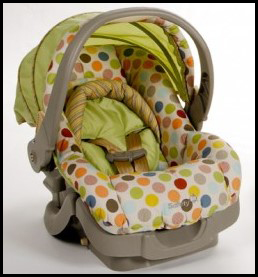
\includegraphics[width=.45\columnwidth]{baby}} 
{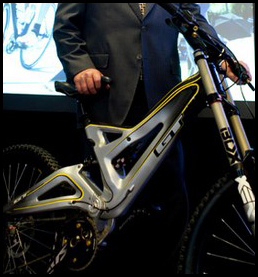
\includegraphics[width=.45\columnwidth]{bike}}}
\vfill
\selectlanguage{american}
\pdfbookmark[1]{StrategicIssues}{StrategicIssues}
\chapter*{Strategic Issues}

\begin{itemize}
  \item Currently have an unrelated portfolio amongst business units.
  \item Competitors have already outsourced to Asia \cite{VoiceofAmerica2009}.
  \item Reduced earnings due to reduced bicycle sales \cite{Symon2014}.
  \item Home Furnishings division is losing revenue YOY.
  \item Unfavorable foreign exchange rates reducing net profits \cite{Symon2014}.
  \item The board believes the company’s market price is currently undervalued.
  \item Finding a way to stay ahead of the competition aside from competing on price.
\end{itemize}

\pdfbookmark[2]{Options}{Options}
\pagebreak
\chapter*{Options}


\begin{enumerate}
  \item Quality vs. Quantity - Return to the company's core value of quality premium products.  Increase R\&D in order to create more innovative products that demand a higher profit margin.  Become the "Apple" of bicycle and juvenile products.
  \item Divest The Core - Divest the home furnishings business in order to increase company focus and investment in Dorel's more successful business units (Recreational/Leisure and Juvenile).
  \item Walk the Online - Begin pushing product sales through an online channel, by selling directly to consumers instead of distributing through retail outlets, decreasing consumer leverage and ideally improving margin potential.
  \item Bjorn to be Wild - Acquire the Baby Bjorn business, a smaller company that focuses on high quality niche products that would also help Dorel enter the Asian-Pacific markets.
\end{enumerate}

\section{Recommendation}
We believe that Dorel's best opportunity for success is to reverse it's current strategy of low-margin low-quality products, and return to it's original core values of safety, quality, and values.  In order to achieve this, Dorel must place a greater emphasis on research \& development, placing quality above everything else.  
\\[2\baselineskip]
\centerline{\includegraphics[scale=0.8]{Guru}}

\selectlanguage{american}

\endgroup			

\vfill

